\documentclass[conference]{IEEEtran}
\IEEEoverridecommandlockouts
% The preceding line is only needed to identify funding in the first footnote. If that is unneeded, please comment it out.
\usepackage{cite}
\usepackage{amsmath,amssymb,amsfonts}
\usepackage{algorithmic}
\usepackage{graphicx}
\usepackage{textcomp}
\usepackage{subcaption}
\usepackage{caption}
\usepackage{xcolor}
\usepackage{float}
\def\BibTeX{{\rm B\kern-.05em{\sc i\kern-.025em b}\kern-.08em
    T\kern-.1667em\lower.7ex\hbox{E}\kern-.125emX}}
\begin{document}

\title{+-\\
%{\footnotesize \textsuperscript{*}Note: Sub-titles are not captured in Xplore and
%should not be used}
}

\author{\IEEEauthorblockN{Miguel Antonio Rodriguez Delgado}
\IEEEauthorblockA{\textit{Electronic Engineering} \\
\textit{\textbf{Hamm-Lippstadt University of Applied Sciences}}\\
Dortmund, Germany \\
miguel-antonio.rodriguez-delgado@stud.hshl.de}
}

\maketitle

\begin{abstract}

Deep learning techniques are growing in all fields, and game playing in not an exception. With this paper we review how different deep learning methods to understand how the can be used in gaming environments. Along this paper we will show how deep learning can be applied for a real world example, focusing in the development of the well known Tic-tac-toe game. We also share the results of the comparison using deep learning techniques against coding the the same game in a classical way.


\end{abstract}

\begin{IEEEkeywords}
Deep learning, Automatic Play Gaming, Tic-tac-toe, Minimax, Neural-networks.
\end{IEEEkeywords}

\section{Introduction}\label{sec:intro}

Video games industry is becoming an important part on people's life, not only by offering entertainment, but also by offering sense of belonging and interconnecting people \cite{niche}. Reports of the Entertainment Software Association (ESA) on 2020 showed that nowadays, and boosted by the corona-virus lockdown  not only young males, but also women, adults and even retired people is attracted by this industry \cite{niche}.

Deep learning algorithms and Artificial Intelligence (AI) have been used in may fields, including the video game industry since 1971, starting with Computer Space and Pong on the Atari 2600 \cite{atari}.

Artificial Intelligence is defined the study of "Intelligent Agents", as any device that can perceive its environment and based on it attempt to take actions to succeed in a goal by maximizing its chances of success \cite{ai}. Machine learning and deep learning algorithms are the tools used to generate these so called intelligent agents \cite{ai}.


\section{Artificial Intelligence On Games}

As described on \ref{sec:intro}, AI has been present in games since the earlies seventies, 
\cite{sony}. However, in the 1957  a team at Carnegie Mellon University predicted that in 1967 a computer would have been capable of defeating a chess world champion \cite{euristic}, but they did not anticipate the hight complexity to predict the correct order of movements required for this task. But at the end of the decade of seventies, a computer defeated for the first time a world champion level chess player \cite{bad}.

In the same way, Artificial Intelligence has been used to defeat humans in other games, such as Mahjong and Go \cite{sony}. These kind of games required a lot of computation and learning algorithm, but they have the possibility to take the time to perform all the necessary calculations. But more advance games, such as Sony's Gran Turismo, have an increased difficulty to master the correct algorithm to drive a race car since many decisions have to be made in real time \cite{sony}.

\section{Chess}\label{sec:chess}

The British mathematician and computer scientist Alan Turing was one of the scientist that developed the first algorithm for playing chess. The design of the algorithm was made to be run on a computer that did not exist at that time \cite{how}.

On 1951 Alan Turing with David Gawen Champernowne deigned a heuristic algorithm and they try to run in on a 1951 Ferranti Mark 1 computer, but due to the limitations of the computational power of the machine the task was impossible for the computer \cite{how}.

Each position on a chess game can be represented as outcome of all the previous positions and moves. For this reason, a chess program do not only need to take into account the current move but the previous and even most important, the possible next moves \cite{how}. In Figure \ref{chess:tree} we can see a tree of how each move can generate a limited number of moves, and how the tree grow deeper after every move, so the chess program can select the best next move \cite{how}

\begin{figure}[h]
\centering
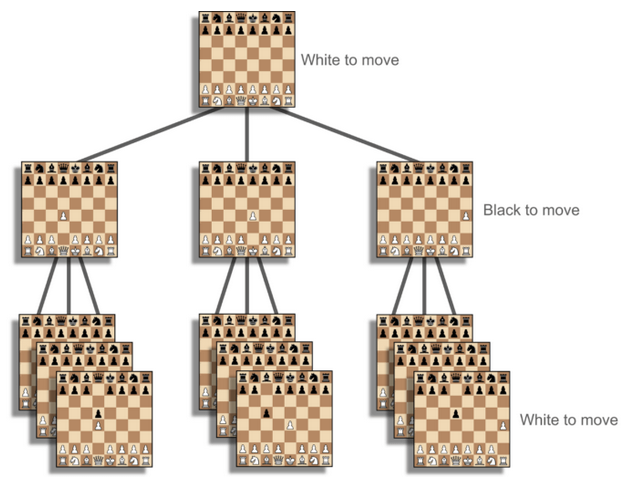
\includegraphics[scale=0.52]{img/tree}
\caption{Searching tree on a chess game \cite{how}}
\label{chess:tree}
\end{figure}

According to Claude Shannon there are two main ways of searching on a chess program, brute-force and selective searches. The first one takes a look at every movement on the board but with a fixed depth of movements, while the second one search for the best candidates going through all the moves and ignore the other branches \cite{how}

Some of the most important algorithms include Chess Challenger, Chessmaster, IBM’s Deep Blue and Alpha-Beta Pruning, but since they will be let out of the scope of this research to focus on Deep Mind, which uses \textit{Residual Policy and Value Networks} and \textit{Reinforcement Learning}

Deep Mind is an artificial intelligence laboratory that have successfully created an algorithm based on reinforcement learning capable to defeat world champions in games as chess, go and shogi \cite{how}.

The algorithm \textit{Alpha Go} is a neural network that defeated for the fist time a Go's world champion, a game that is significantly more complex than chess. Alpha Go was trained using human data and due to its success, it was object of the award-winning documentary \cite{how}. Alpha Zero, its successor, defeated Alpha Go with a score of 100 - 0 games, but Alpha Zero was trained with no human data a it uses less computational power \cite{how}.

Alpha Zero generalizes a network to play three different games, chess, go and shogi. The Alpha Zero algorithm uses reinforcement learning, a field of deep learning that gives rewards for winning or uses penalties for losing in the environment emphasising self-playing \cite{how}

The foundation of most popular neural networks are the \textit{Residual Networks}. These networks let us decode and encode information in the data. One of the advantages of these structures is that the gradient signal regarding the loss function can travel further, allowing a deeper neural network training \cite{how}. These kind of networks to predict the next move, enhances the future maps, information that can be used to improve the present position and move \cite{how}. Also, another kind of networks, \textit{Policy Networks}, select the best possible network and search deeper through the tree, which added with the Residual network limits the searching space and time \cite{how}

There are three machine learning paradigms, \textit{supervised learning, unsupervised learning} and \textit{reinforcement learning} \cite{how}. This last one focuses on providing rewards or penalties from an specific environment during the learning process \cite{how}. In Figure \ref{chess:reinforcement} we can see an example of reinforcement learning. In this example an agent performs an action 

\begin{figure}[h]
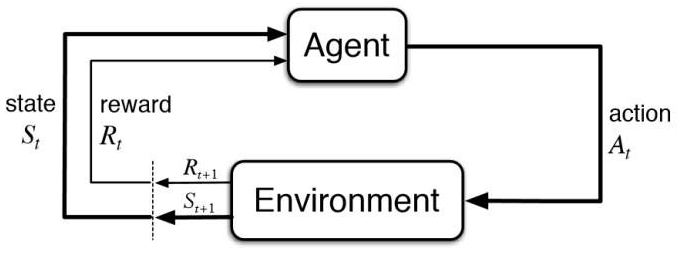
\includegraphics[scale=0.5]{img/deepchess}
\caption{Reinforcement learning on Deep Main algorithm \cite{how}}
\label{chess:reinforcement}
\end{figure}

\section{Racing games}

Since the introduction of deep learning for racing games, reinforcement learning and supervised learning have been the two principal ways to train a network to learn how to drive a car \cite{racingpdf}.

For the reinforcement learning process, the computer learns on its own by trial and error \cite{racingpdf}. Consequently, it is not required to have a big set of data before starting with the training \cite{racingpdf}. The most important attributes to train a network with reinforcement learning are an agent and an environment \cite{racingpdf}. The agent takes different actions taking into account the different states of the environment, and the environment, depending on the actions the agent can get different rewards, and then the states of the environment change \cite{racingpdf}. This is performed in a cycle indefinitely. 

The goal of the agent is to maximize the rewards. However, this is not always the best way to train a racing game network, for instead, the reward assignment. Many times the algorithm can perform an action that lead to a positive or negative reward in previous cycles, or many steps ago, and this will make difficult for the algorithm to learn from these actions \cite{racingpdf}. Another problem is the so called "explore-exploit-dilemma". This problem leads to get stuck at a low score, the local minimum, without knowing that it can perform better \cite{racingpdf}.

For the supervising learning process, the machine uses a known dataset to learn from it and to generate predictions \cite{racingpdf}. The training data set is made up of different examples, including a input object and a desired result value \cite{racingpdf}. The goal for the supervising learning process is to generate a inferred function that will correctly determine and generalize the output even for unseen instances in a reasonable way \cite{racingpdf}  

\section{GTSophy}

Gran Turismo, a racing simulation video game, made its debut in 1997 and has sold over 80 million units \cite{sony}, making this one of the most famous racing games. Grand Tursimo Sophy or GTSophy is an artificial intelligence agent created by Sony and it was aimed to defeat the best human racing players \cite{sony}. For this development Sony made use of fundamental AI researches, using a hyper-realistic real racing world simulator, and an infrastructure for massive scale artificial intelligence training \cite{sony}.

The first interaction between Sophy and a human players was in July 2021. In that moment Sophy raced against four of the best Gran Turismo players, and learned from the race \cite{sony}. After this, according to Sony, it took about 20 PlayStations running simultaneously during 12 days to train Sophy, for its first race to a "superhuman level" \cite{sony}.

As we discussed in section \ref{sec:chess}, artificial intelligence have been used to defeat humans in games as chess and go, but according to Sony \cite{sony}, generating a AI algorithm to drive a racing car represented a huge challenge since many decisions have to done in real time. By October 2021 Gran Turismo Sophy defeated and outperformed the best human Gran Turismo drivers \cite{sony}.

According to Sony, there are many games with different challenges to research on artificial intelligence and deep learning algorithms. For this reason Sony wants to apply learnings in other Sony games \cite{sony}

\section{Minmax}

In game theory, Minmax is a decision method that aims to minimize the maximal possible loss in games against an adversary and with perfect information \cite{nature}. Minmax is a recursion algorithm that can be summarized as the choice of the best move on the assumption that the opponent will choice the worst possible movement for you \cite{nature}.

The French mathematician Emile Borel was the first person in propose a rigorous method for competitive games back in 1921, and to study the applicable strategies on the zero-sum games \cite{nature}. However, it was John von Neumann who published the Minmax concept Zur Theorie der Gesellschaftsspiele, \textit{"About the theory of society games"} \cite{nature}.

According to von Neumann, a game is a conflictive situation where each person takes a decision knowing that the others will also take different decisions, and the result of the conflict is determined on the taken decisions \cite{nature}. Based on this we can infer that each player knows its opponent strategy, and he should take into account all the possible responses from the opponent, and the maximum loss that the movement can bring \cite{nature}. Then the player, with the information of the minimal maximal loss select his move \cite{nature}.

In games with non-zero-sum, both the minimax and the maximin strategies have to be used \cite{nature}. The first one tries to minimize the opponent overcome, and the second one tries to improve its own success \cite{nature}.

In figure \ref{chess:minmax} we can see how a tree of possible moves is constructed. For this example the A position will search for the maximiser, in the second line the algorithm will search for the minimizer on positions B and C, in the next line again the maximizer for positions D, E, F, and G and so on.

\begin{figure}[H]
\centering
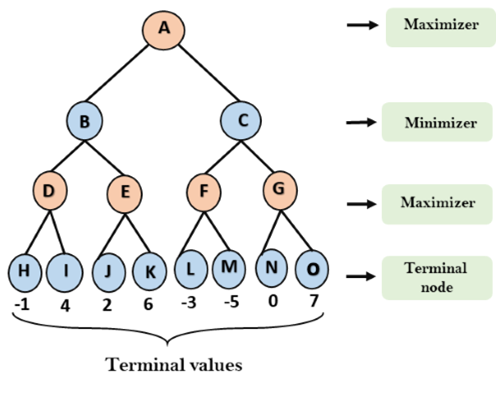
\includegraphics[scale=0.55]{img/minmax.png}
\caption{Minmax algorithm structure}
\label{chess:minmax}
\end{figure}

Chess is one of the games where the minimax algorithm is used. In this case it is used an evaluation function to estimate the value of the position at a given depth \cite{alphatoe}. In a similar way that we showed in Figure \ref{chess:minmax}, a massive three has to be created to analyse the possibles outcome of a determinate move, but the tree can be huge since in chess we can get up to $10^123$ possible positions and this will represent a problem both for processing time and for storage \cite{alphatoe}. Instead, to solve this problem, the algorithm can take an estimation based on the next 8 moves, to check how good a position \cite{alphatoe}. In chess there is an easy way to calculate how good a move is, for example, having more pieces on the board can lead to an advantage and also giving a value to the different pieces where for example a bishop is worth two pawns \cite{alphatoe}.

However, minimax algorithm is not a good solution for games as Go since the state space is too big. To solve this problem, an algorithm such as Monte Carlo sampling can be used \cite{alphatoe}.

\section{Monte Carlo Sampling}

There are three main problems why minimax can not be used on games as Go. First as stated in the section before, the state space is huge, at the beginning of the game there are already 360 possible moves; second, there are not very good evaluation functions, most of the times there is not a way to evaluate how good or bad a position is until the end of the game; and third, Go is difficult to learn even for humans \cite{alphatoe}.

To face this problem, the simplest algorithm we can use is Monte Carlo Sampling. Monte Carlo Sampling do not make use of an evaluation function \cite{alphatoe}. Instead, as we can see in Figure \ref{chess:montecarlo}, Monte Carlo algorithm select a random position, and from that position we make random moves for different positions until the end of the game, and when the end is reached we can check if we won or lost, and the result would be the average result of the simulation.

\begin{figure}[!h]
\centering
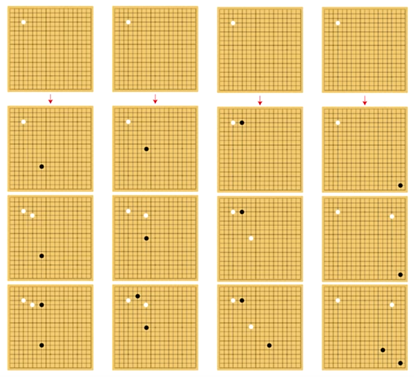
\includegraphics[scale=0.55]{img/montecarlo.png}
\caption{Montecarlo algorithm structure}
\label{chess:montecarlo}
\end{figure}

\section{Drawbacks}

The introduction of artificial intelligence and deep learning algorithms do not only offer advantages in the different fields that we have talk about in the previous sections, but it also brings different risks. Since the focus of study of this paper is gaming, an example on how AI can represent a risk in the development of a chess software that can identify unique styles of playing and it is able to point out with no previous information, who it is playing with, what represent a serious privacy risk \cite{unmask}.

\section{Case Of Study - Tic-Tack-Toe}

For the purpose of this paper, I have selected the known Tic Tac Toe as the game for study case, since it is a simple game with not too many possibilities, and it is known for most of the people.

To simplify the explanation of the algorithm we will star in the position described of Figure \ref{tic:p1} \cite{tictac}. At this point we can assume that player "X" started and has played three times and "O", was the second player and has also played three times. This will allow us to check only a few possibilities instead of checking the whole range of options.

\begin{figure}[H]
\centering
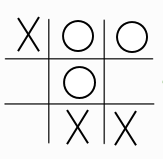
\includegraphics[scale=0.55]{img/chess1.png}
\caption{Tic Tac Toe game example for minimax algorithm development}
\label{tic:p1}
\end{figure}

After the position showed in Figure \ref{tic:p1}, player "X" will have three options to play, as shown in Figure \ref{tic:p2}. If "X" plays in the left middle position as showed in Figure \ref{tic_2.1}; or in the right middle position as in Figure \ref{tic_2.3} the game can continue; if player "X" plays in the position showed in Figure \ref{tic_2.2}, the game will end and "X" will win. For a human this will be the obvious move, but for a PC this might not be the case, so in this case the algorithm will analyse the outcome of all possible moves.

\begin{figure}[H]
\centering
\begin{subfigure}{.24\textwidth}
    \centering
    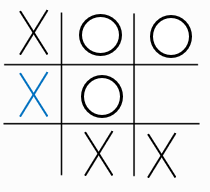
\includegraphics[scale=0.45]{img/chess2_1.png}
    \caption{"X" First optional move}
    \label{tic_2.1}
\end{subfigure}
\begin{subfigure}{.24\textwidth}
    \centering
    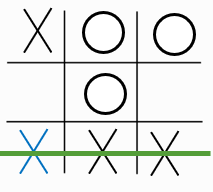
\includegraphics[scale=0.45]{img/chess2_2.png} 
    \caption{"X" Second optional move}
    \label{tic_2.2}
\end{subfigure}
\begin{subfigure}{.24\textwidth}
    \centering
    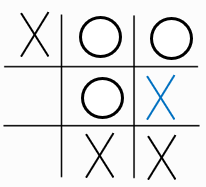
\includegraphics[scale=0.45]{img/chess2_3.png}
    \caption{"X" Third optional move}
    \label{tic_2.3}
\end{subfigure}
\caption{Possible option move for solving Tic tac toe example.}
\label{tic:p2}
\end{figure}

If player "X" plays in the positions showed in blue color in Figure \ref{tic_2.1} or in Figure \ref{tic_2.3}, player "O" will now have to play. All the possible outcomes for player "O" are shown in figure \ref{tic_3}. Starting from position on Figure \ref{tic_2.1} "O" can take two possible options, the one on the left bottom corner Fig. \ref{tic3_1}, which leads "O" to win; or the on the right middle Fig \ref{tic3_2}, that will give a last option for player "X" to play. If player "X" played as in Figure \ref{tic_2.1}, player "O" can play in the left middle, giving "X" a last option to play or can play on the bottom left winning the game. 


\begin{figure}[H]
\centering
\begin{subfigure}{.24\textwidth}
    \centering
    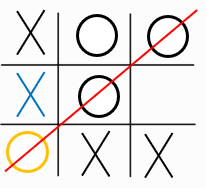
\includegraphics[scale=0.45]{img/chess3_1.png}
    \caption{First optional move}
    \label{tic3_1}
\end{subfigure}
\begin{subfigure}{.24\textwidth}
    \centering
    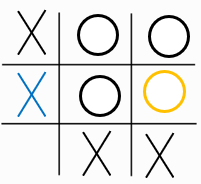
\includegraphics[scale=0.45]{img/chess3_2.png} 
    \caption{Second optional move}
    \label{tic3_2}
\end{subfigure}
\begin{subfigure}{.24\textwidth}
    \centering
    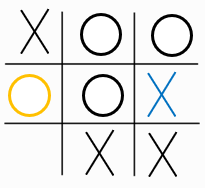
\includegraphics[scale=0.45]{img/chess3_3.png}
    \caption{Third optional move}
    \label{tic3_3}
\end{subfigure}
\begin{subfigure}{.24\textwidth}
    \centering
    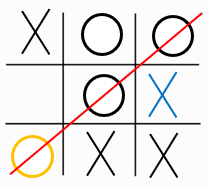
\includegraphics[scale=0.45]{img/chess3_4.png}
    \caption{Third optional move}
    \label{tic3_4}
\end{subfigure}
\caption{Possible moves of the opponent.}
\label{tic_3}
\end{figure}

Finally, in Figure \ref{atic4} we have the last two options, in both of the options showed in 

\begin{figure}[H]
\centering
\begin{subfigure}{.24\textwidth}
    \centering
    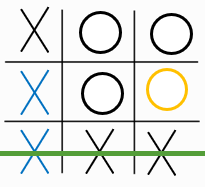
\includegraphics[scale=0.45]{img/chess4_1.png}
    \caption{"X" play after figure \ref{tic3_2}}
    \label{atic4_1}
\end{subfigure}
\begin{subfigure}{.24\textwidth}
    \centering
    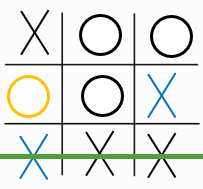
\includegraphics[scale=0.45]{img/chess4_2.png} 
    \caption{"X" play after figure \ref{tic3_3}}
    \label{atic4_2}
\end{subfigure}
\caption{Possible option move for solving Tic tac toe example.}
\label{atic4}
\end{figure}

With this information the minimax algorithm can start to analyse the best move. Since the minimax algorithm is based on which result would give the better score, we have to analyse the score given in all the possibilities, as stated before, a human can easily decide on the one move that will win the game, but for a computer is not that simple. For this, we will give three possible scores for the three possible outcomes on a Tic tac toe game, if "X" wins we will give a result of +1, if there is a tie the result will be 0 and if "O" wins the result will be -1.

With these scores we can easily give a score of +1 to the position \ref{tic_2.2}, but we cannot give any scores to the positions in figure \ref{tic_2.1} or figure \ref{tic_2.3}. To give a score to these positions we will have to go down in the three of solutions, and then we can give a result of -1 to the positions in figures \ref{tic3_1} and \ref{tic3_4}, finally we can give a result of +1 to the two positions in figure \ref{atic4}.

The minimax algorithm will always assume that the opponent will take the best possible move for him, from here the minimax name comes \cite{tictac}. From the third turn game will select the +1, but for the second turn game, when "O" plays, the given result will be -1, since it will select the minimum value. At this point the three values will be -1 for \ref{tic_2.1} and \ref{tic_2.3} and +1 for \ref{tic_2.2}, selecting the last position as the move to take.

\section{Conclusion}

Video games are an important industry nowadays, and with more technology and more demanding games, artificial intelligence and deep learning will play an important roll in the development of virtual opponents in all kind of games. In this paper we have only discussed some of the easiest algorithms to implement, but we have also see how an algorithm can be used to take a decision on a simple game.

All the different games represent a different challenge to implement a virtual agent or opponent, and therefore, there will be a huge field to research in the specific area of deep learning for video games.


\begin{thebibliography}{00}

\bibitem{niche} Lugris, M. (2020, July 25). New ESA Report Shows Gaming Is No Longer A Niche Market. TheGamer. https://www.thegamer.com/esa-gaming-niche-popular-die-mad-gamers/

\bibitem{atari} Skinner, G.,  $\&$ Walmsley, T. (2019, February). Artificial intelligence and deep learning in video games a brief review. In 2019 IEEE 4th International Conference on Computer and Communication Systems (ICCCS) (pp. 404-408). IEEE.

\bibitem{ai} Ongsulee, P. (2017, November). Artificial intelligence, machine learning and deep learning. In 2017 15th international conference on ICT and knowledge engineering (ICT$\&$KE) (pp. 1-6). IEEE.

\bibitem{euristic} A. Newell and H. Simon, “Heuristic Problem-Solving: The Next Advance in Operation Research,” Operations Research, Vol. 6, No. 6, 1958. 

\bibitem{bad} Hapgood, Fred. "Computer chess bad-human chess worse". New Scientist. pp. 827–830. (23–30 December 1982) Retrieved 22 January 2015.

\bibitem {how}How does AI play chess? (2022, September). Baeldung. https://www.baeldung.com/cs/ai-chess

\bibitem{sony} Mukherjee, S. (2022, February 9). Sony’s new AI beats humans in Gran Turismo racing game. Reuters. https://www.reuters.com/technology/sonys-new-ai-beats-humans-gran-turismo-racing-game-2022-02-09/

\bibitem{racing} Lecchi, S. (2009, September). Artificial intelligence in racing games. In 2009 IEEE Symposium on Computational Intelligence and Games (pp. 1-1). IEEE.

\bibitem{racingpdf} Teigar, H., Storožev, M., $\&$ Saks, J. (2017). 2D Racing game using reinforcement learning and supervised learning.

\bibitem{automated} Hutter, F., Kotthoff, L., $\&$ Vanschoren, J. (2019). Automated machine learning: methods, systems, challenges (p. 219). Springer Nature.

\bibitem{wild} Stadelmann, T., Amirian, M., Arabaci, I., Arnold, M., Duivesteijn, G. F., Elezi, I., $\&$ Tuggener, L. (2018, September). Deep learning in the wild. In IAPR Workshop on Artificial Neural Networks in Pattern Recognition (pp. 17-38). Springer, Cham.

\bibitem{unmask} Hutson, M. (2022). Artificial intelligence unmasks anonymous chess players. Science, 129, 129.

\bibitem{alphatoe} Data Science Festival. (2016, September 30). Alpha Toe: Using Deep learning to master Tic-Tac-Toe - Data Science Festival. YouTube. https://www.youtube.com/watch?v=Meb5hApAnj4

\bibitem{nature} Beal, Donald F. (1999). The Nature of Minimax Search. Universidad de Maastricht: Institute of Knowledge and Agent Technology, UM. ISBN 90-62-16-6348.

\bibitem{tictac} The Coding Train. (2019, December 11). Coding Challenge 154: Tic Tac Toe AI with Minimax Algorithm. YouTube. https://www.youtube.com/watch?v=trKjYdBASyQ


\end{thebibliography}
\end{document}
